\begin{frame}{Transferencia del GNC a la ADRES*}
\begin{center}
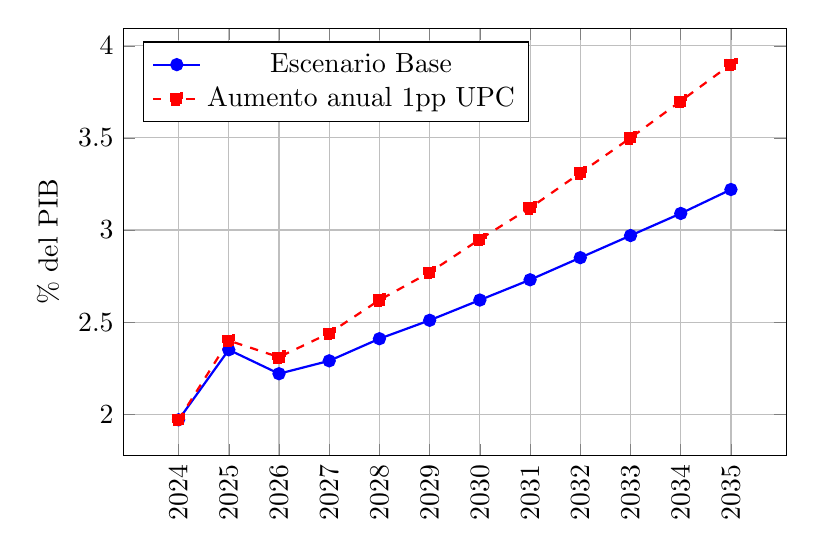
\begin{tikzpicture}
    \begin{axis}[
        width=10cm, height=7cm,
 %       xlabel={Año},
        xlabel style={yshift=-15pt},
        ylabel={\% del PIB},
        xtick=data,
        grid=major,
        xticklabels={2024, 2025, 2026, 2027, 2028, 2029, 2030, 2031, 2032, 2033, 2034, 2035},
        xticklabel style={rotate=90, anchor=east},
        legend pos=north west,
        ymajorgrids=true,
        legend style={at={(0.03,0.97)}, anchor=north west}
    ]
    
    % Escenario Base
    \addplot[thick, color=blue, mark=*] coordinates {
        (2024,1.97) (2025,2.35) (2026,2.22) (2027,2.29) (2028,2.41) 
        (2029,2.51) (2030,2.62) (2031,2.73) (2032,2.85) (2033,2.97) 
        (2034,3.09) (2035,3.22)
    };
    \addlegendentry{Escenario Base}
    
    % Choque +1pp UPC
    \addplot[thick, color=red, mark=square*, style=dashed] coordinates {
        (2024,1.97) (2025,2.40) (2026,2.31) (2027,2.44) (2028,2.62) 
        (2029,2.77) (2030,2.95) (2031,3.12) (2032,3.31) (2033,3.50) 
        (2034,3.70) (2035,3.90)
    };
    \addlegendentry{Aumento anual 1pp UPC}
    
    \end{axis}
\end{tikzpicture}
\\{\footnotesize * No incluye los 4,4 puntos del antiguo CREE}%\\
\end{center}
%\vspace{0.1cm}
%{\footnotesize \textit{Fuente: Marco Fiscal de Mediano Plazo 2024, Ministerio de Hacienda.}}
\end{frame}
